\newpage
\section{The Medium Access Control(MAC) Sublayer}
网络连接分两种: P2P or Broadcasting

MAC 是 Broadcasting. 

\subsection{The Channel Allocation Problem}
Static channel allocation: FDMA (bandwidth 分 $N$ 等大的块, 每个人一块)

但网络有 bursty (突发性), 所以使用 Dynamic channel allocation, also called Statistical Multiplexing. 


\subsubsection{Preliminary Queueing Theory}
\begin{align*}
    T_N=\frac{1}{\mu (C/N)-(\lambda/N)}=\frac{N}{\mu C-\lambda}=NT
\end{align*}
\begin{itemize}
    \item Consider any system that has a capacity $C$, the maximum rate at which it can perform work
    \item Assume that $R$ represents the average rate at which work is demanded from this system.
\end{itemize}

If $R<C$, 系统可以处理工作, 但因为有 the irregularity of the demands, 所以还是不行. If $R>C$, 系统寄. 

Two unpredictable sources lead to the irregularity of the demands:
\begin{enumerate}
    \item the arrival times
    \item the service times
\end{enumerate}


Queueing Theory: the characterization of the arrival times and the service times and the evaluation of their effect on queueing phenomena form the essence of queueing theory.

Let $C_n$ denote the $n$-th customer to arrive at a queueing facility, and 
\begin{itemize}
    \item $\tau_n=$ arrival time for $C_n$
    \item $t_n=\tau_n-\tau_{n-1}=$ interarrival time between $C_n$ and $C_{n-1}$
    \item $x_n=$ service time for $C_n$. 
\end{itemize}
$\{ t_n\}$,  $\{ \tau_n \}$ 是随机变量且独立分布. 定义两个一般随机变量:
\begin{itemize}
    \item $\tilde{t}=$ interarrival time
    \item $\tilde{x}=$ service time
\end{itemize}

probability distribution function (PDF)
\begin{itemize}
    \item $A(t)=P[\tilde{t}\le t]$
    \item $B(x)=P[\tilde{x}\le x]$
\end{itemize}

probability density function (pdf)
\begin{itemize}
    \item $a(t)=\frac{d A(t)}{dt}$
    \item $b(x)=\frac{d B(x)}{dx}$
\end{itemize}

important moments 联系这些随机变量
\begin{itemize}
    \item $E[\tilde{t}]=$ mean interarrival time $=\frac{1}{\lambda}$, where $\lambda$ is the average arrival rate. 
    \item $E[\tilde{x}]=$ mean service time $=\frac{1}{\mu}$. 
\end{itemize}

The study of queues naturally breaks into three cases:
\begin{enumerate}
    \item elementary queueing theory
    \item intermediate queueing theory
    \item advanced queueing theory
\end{enumerate}
根据 $a(t)$ 与 $b(x)$ 区分. 

A three-component description $A/B/m$, which denotes 
\begin{itemize}
    \item $m$-server queueing system
    \item $A$ the interarrival time distribution
    \item $B$ the service time distribution
\end{itemize}

And distributions symbols:
\begin{itemize}
    \item $M$ = exponential (i.e. Markovian)
    \item $Er$ = r-stage Erlangian
    \item $Hr$ = r-stage Hyperexponential
    \item $D$ = Deterministic
    \item $G$ = General
\end{itemize}

The simplest interesting system is the $M/M/1$ queue. 

\paragraph{General Results} The most important system parameter for $G/G/1$ is the utilization
factor $\rho$, 
\begin{align*}
    \rho=\lambda\tilde{x}
\end{align*}
单个 server 单位时间处于忙碌状态的时间. $\rho$ is the expected fraction of the system's capacity that is in use.

For multiple-server system $G/G/m$ 
\begin{align*}
    \rho=\frac{\lambda\tilde{x}}{m}
\end{align*}

In all cases a stable system is one for which $0\ge \rho<1$. 

The closer $\rho$ approaches unity, the larger are the queues and the waiting time.

The average time in system
\begin{align*}
    T=\tilde{x}+W
\end{align*}
where $W$ is waiting time in queue. 


\paragraph{Little's Result} 系统中平均客户数
\begin{align*}
    \bar{N}=\lambda T
\end{align*}

The average queue size is 
\begin{align*}
    \bar{N}_q=\lambda W
\end{align*}

In $G/G/m$, these quantities are related by
\begin{align*}
    \bar{N}_q=\bar{N}-m\rho
\end{align*}
可以理解为系统中平均客户数减去正在被服务的客户数就是正在等待服务的客户数了

动态客流:
\begin{itemize}
    \item $E_k$ $k$ customers 在系统中的状态
    \item $P_k(t)=P[N(t)=k]$ 在 $t$ 时, 系统处于 $E_k$ 的概率
    \begin{align*}
        \frac{dP_k(t)}{dt}=
    \end{align*}
\end{itemize}

Consider a stable system, $\displaystyle p_k=\lim_{t\to0} P_k(t)$. 

The $M/M/1$ queue: 
\begin{itemize}
    \item This system has a Poisson input. 
    \item The probability $P_k(t)$ of $k$ arrivals in an interval whose duration is $t$ sec is given by
    \begin{align*}
        P_k(t)=\frac{(\lambda t)^k}{k!}e^{-\lambda t}
    \end{align*}
    \item The average number of arrivals during this interval is
    \begin{align*}%TOOD 15
        \bar{N}(t)=\sum_{k=0}^{\infty} kP_k(t)=\lambda t
    \end{align*}
    So the average arrival rate in a unit time is $\lambda$.
    \item The average service time is $\tilde{x}=\frac{1}{\mu}$
    \item The probability of having $k$ customers in the system is given by
    \begin{align*}
        p_k=(1-\rho)\rho^k
    \end{align*}
    \item The average number in the system is
    \begin{align*}
        \bar{N}=\sum_{k=0}^\infty kp_k=\frac{\rho}{1-\rho}
    \end{align*}
    \item Using Little's result and the average time in the system $T$ is
    \begin{align*}
        T=\frac{\bar{N}}{\lambda}=\frac{\frac{1}{\mu}}{1-\rho}
    \end{align*}
    \item $W$ is
    \begin{align*}
        W&=\frac{\bar N_q}{\lambda}=\frac{\frac{\rho}{\mu}}{1-\rho}\\
        \bar N_q&=\bar N -m\rho =\frac{\rho^2}{1-\rho}
    \end{align*}
\end{itemize}

\subsubsection{The Performance of Static FDM}
The mean time delay $T$ to send a frame onto a channel of capacity $C$ bps (Note only one channel here). Assume
\begin{itemize}
    \item the average arrival rate $\lambda$
    \item the average length  $\frac{1}{\mu}$
    \item the service rate $\tilde{x}=\frac{1}{\mu C}$
    \item The utilization factor $\rho=\lambda\tilde{x}$
    \item According to the results of the $M/M/1$ queue
    \begin{align*}
        T=\frac{\frac{1}{\mu C}}{1-\rho}=\frac{1}{\mu C-\lambda}
    \end{align*}
\end{itemize}

Let us divide the single channel into $N$ independent subchannels, each with capacity $C/N$ bps. For subchannels:
\begin{itemize}
    \item mean input rate $\frac{\lambda}{N}$
    \item According to the results of an $M/M/m$ queue, the mean time delay
    \begin{align*}
        T_N=\frac{1}{\mu(C/N)-(\lambda /N)}=\frac{N}{\mu C-\lambda}=NT
    \end{align*}
\end{itemize}
分别排队等待时间更长. 

\subsubsection{Key Assumptions of Dynamic Channel Allocation}
Five key assumptions:
\begin{enumerate}\small
    \item Independent Traffic: The model consists of N independent stations. 每个人收发信号随机且独立. 
    \item Single Channel: A single channel is available. 所以可能有冲突. 
    \item Observable Collisions: All stations can detect the collision when it occurred. 
    \item Continuous or Slotted Time: Frame transmission can begin at any instant, or must begin at the start of a slot. (连续 or 有时钟)
    \item Carrier Sense or No Carrier Sense: (发送前是否检测信道状态) 
    \subitem With the carrier sense assumption, stations can tell if the channel is in use before trying to use it.
    \subitem If there is no carrier sense, stations cannot sense the channel before trying to use it. 
\end{enumerate}

\subsection{Multiple Access Protocols}
\subsubsection{ALOHA}
Each user terminal sharing the same upstream frequency to send frames to the central computer.

Two versions of ALOHA: pure and slotted.

\subsubsection{Pure ALOHA}
sender 向 central computer 发 frame, 然后 central computer rebroadcasts the frame to all of the stations, sender 监听这个转播来确定是否发送成功. (收到的frame 需要 和 发送的一致) 如果发送失败, sender 等待随机时间后再次发送. 

\begin{figure}[!htb]
    \centering
    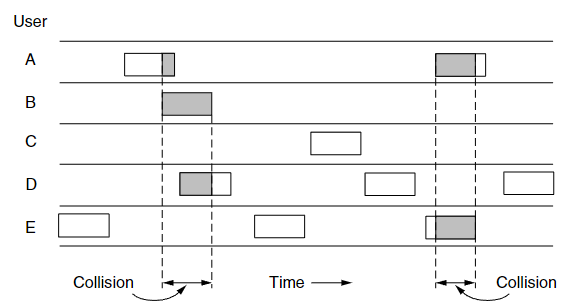
\includegraphics[width=0.309\textwidth]{pic/CN4/pure ALOHA.png}
    \caption{In pure ALOHA, frames are transmitted at completely arbitrary times.}
\end{figure}
If the first bit of a new frame overlaps with just the last bit of a frame that has almost finished, both frames will be totally destroyed.

An interesting question is: what is the efficiency of an ALOHA channel?
\begin{itemize}
    \item a Poisson distribution
    \item with mean of $N$ new frames per frame time. % (ppt) 中是 N
    \subitem If $N>1$, 超过信道容量, 寄. 
    \subitem expect $0<N<1$ 
    \item with mean of $G$ old frames per frame time.
    \subitem $G\ge N$
    \subitem At load low ($N\approx 0$), $G\approx N$
    \subitem At high low, $G>N$
    \subitem the throughput $S=GP_0$,  $P_0$ is the probabilityof a transmission succeeding

    \begin{figure}[!htb]
        \centering
        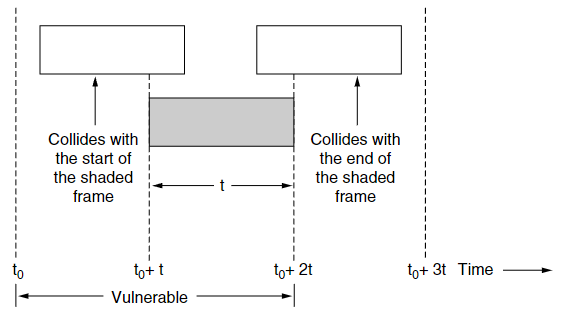
\includegraphics[width=0.309\textwidth]{pic/CN4/Vulnerable period for the shaded frame}
        \caption{Vulnerable period for the shaded frame}
    \end{figure}
    对一帧要保证 $2t$ 时间内没有其他帧发送. 
    \item The probability that $k$ frames are generated during a given frame time
    \begin{align*}
        P[k]=\frac{G^ke^{-G}}{k!},\ G\sim \lambda t
    \end{align*}
    \subitem The probability of zero frames is $e^{-G}$
    \subitem the entire vulnerable period is $P_0=e^{-2G}$
\end{itemize}

\begin{figure}[!htb]
    \centering
    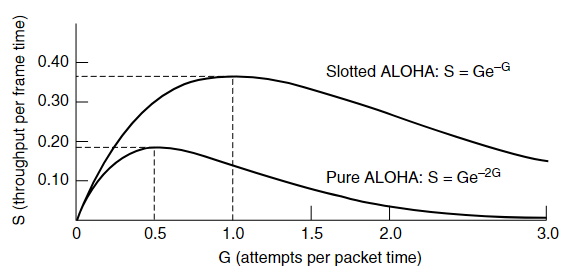
\includegraphics[width=0.309\textwidth]{pic/CN4/Throughput versus offered traffic for ALOHA systems.}
    \caption{Throughput versus offered traffic for ALOHA systems.}
\end{figure}
pure ALOHA 的最值在 $G=0.5$ 处.  Slotted ALOHA 的在 $G=1$ 处. 

\subsubsection{Slotted ALOHA}
divide time into discrete intervals called slots, agree on slot boundaries: 帧只能在 slot 的起点发. 

The probability of no other traffic is $e^{-G}$, so $S=Ge^{-G}$. The probability of a collision is  $1-e^{-G}$. 

推导:
\begin{itemize}
    \item The probability of a transmission requiring exactly $k$ attempts is
    \begin{align*}
        P_k=e^{-G}(1-e^{-G})^{k-1}
    \end{align*}
    \item The expected number of transmissions $E$ is
    \begin{align*}
        E=\sum_{k=1}^\infty kP_k=e^G
    \end{align*}
\end{itemize}
As a result of the exponential dependence of $E$ upon $G$, small increases in the channel load can drastically reduce its performance.

\subsubsection{Carrier Sense Multiple Access(CSMA) Protocols}
With slotted ALOHA, the best channel utilization that can be achieved is $1/e$. 因为任意发送太容易导致冲突了. 

\paragraph{1-persistent CSMA} 先监听信道看是否空闲, 空闲就发送, 不空闲一直侦听直到信道空闲然后发送. 遇到冲突仍然是等待随机时间再执行. The protocol is called 1-persistent because the station transmits with a probability of 1 when it finds the channel idle. 

\paragraph{Nonpersistent CSMA} 先监听信道看是否空闲, 空闲就发送, 不空闲等待随机时间然后再重复算法. 

\paragraph{p-persistent CSMA} applies to slotted channels. 先监听信道看是否空闲,空闲有 $p$ 概率发送, $1-p$ 概率不发送, 等待下一个slot. 不空闲就等待下一个 slot 

\begin{figure}[!htb]
    \centering
    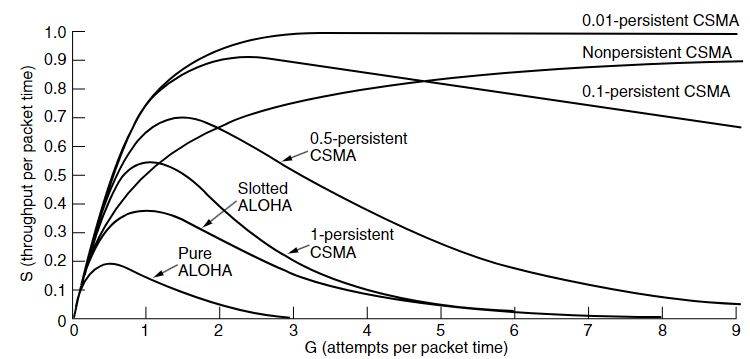
\includegraphics[width=0.309\textwidth]{pic/CN4/Comparison of the channel utilization}
    \caption{Comparison of the channel utilization versus load for various random access protocols.}
\end{figure}


\subsubsection{CSMA with Collision Detection}
Collision detection 边发送边读取. 若读的数据与发的一样就继续, 否则就是产生冲突, 中止发送. 

\begin{figure}[!htb]
    \centering
    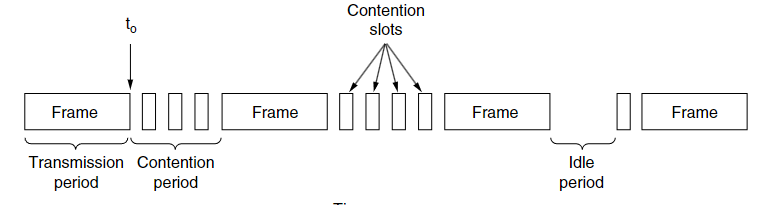
\includegraphics[width=0.42\textwidth]{pic/CN4/CSMA CD}
    \caption{CSMA/CD can be in contention, transmission, or idle state}
\end{figure}

Suppose that two stations both begin transmitting at exactly time $t_0$. How long will it take them to realize that they have collided?
\begin{itemize}
    \item Consider the worst-case scenario. propagate between the two farthest stations is $\tau$
    \item 在 $t_0$ A 发送, 在 $t_0 + \tau -\epsilon$ 时 B 发送, 直到 $2\tau-\epsilon$ 冲突才被 A 探测. 
\end{itemize}
We can think of CSMA/CD contention as a slotted ALOHA system with a slot width of $2\tau$.  

\subsubsection{Collision Free Protocols}
若 the bandwidth-delay product 大, 冲突影响大. 所以来些 没有冲突的算法. 

\paragraph{A Bit-Map Protocol --- Reservation Protocol} $N$ slots, 当作 bit map, bit 1 是发, 仅一个 1 时才发. 但不支持过大的网络. 
\begin{figure}[!htb]
    \centering
    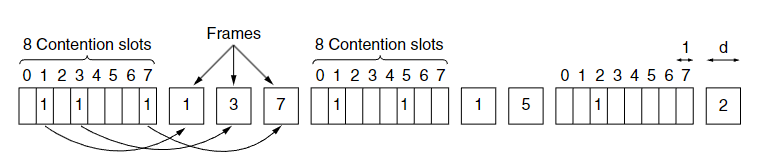
\includegraphics[width=0.42\textwidth]{pic/CN4/The basic bit-map protocol}
    \caption{The basic bit-map protocol}
\end{figure}

\paragraph{Token Passing}令牌轮询, 只有拿到令牌才能发送数据. 但令牌产生与销毁会导致不公平. 
\begin{figure}[!htb]
    \centering
    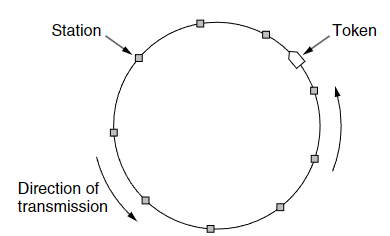
\includegraphics[width=0.309\textwidth]{pic/CN4/Token ring}
    \caption{Token ring}
\end{figure}

\paragraph{Binary Countdown}结合前两方法的优点. 每个站点给个编号, 更大的站点发. 

\subsubsection{Limited-Contention Protocols}
Two important performance measures broadcast network:
\begin{itemize}
    \item delay at low load
    \item channel efficiency at high load.
\end{itemize}


Limited-contention Protocols combine the best properties of the contention and collision-free protocols.
\begin{itemize}
    \item 每个站点有 $p$ 概率获得信道
    \item 但一个站点获得信道, 其他所有站点有 $1-p$ 不获得信道. The value is $kp(1-p)^{k-1}$
\end{itemize}
when $p=\frac{1}{k}$, the value is max. 
\begin{align*}
    Pr[\text{success with optimal} p]=\left( \frac{k-1}{k} \right)^{k-1}
\end{align*}

\begin{figure}[!htb]
    \centering
    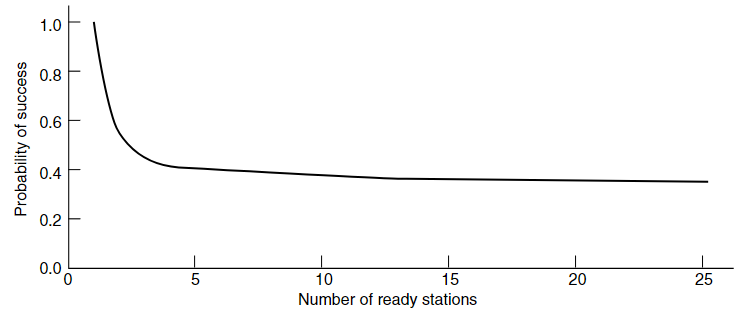
\includegraphics[width=0.42\textwidth]{pic/CN4/Acquisition probability for a symmetric contention channel}
    \caption{Acquisition probability for a symmetric contention channel}
\end{figure}
As soon as the number of stations reaches 5, the probability has dropped close to its asymptotic value of $1/e$.

所以将用户分组, group $x$ 竞争 slot $x$, 成功发送, 失败不发. 合适分组可以降低竞争程度. low load with big group, high load with small group. 


\paragraph{The Adaptive Tree Walk Protocol}结点1 是所有用户, 冲突后会分结点, 进行DFS, 成功会进行 BFS. 
\begin{figure}[!htb]
    \centering
    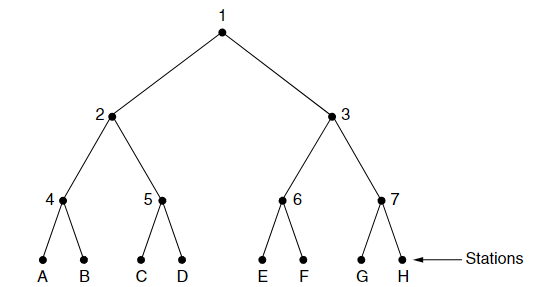
\includegraphics[width=0.309\textwidth]{pic/CN4/The tree for eight stations}
    \caption{The tree for eight stations}
\end{figure}


\subsubsection{Wireless LAN Protocols}
Wireless is more complicated than the wired case
\begin{itemize}
    \item Nodes may have different coverage areas. 
    \subitem 不同结点覆盖区域不同, 要避免之间的冲突. 
    \begin{figure}[!htb]
        \centering
        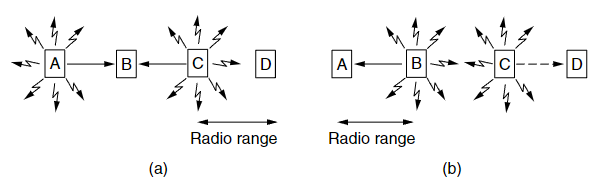
\includegraphics[width=0.42\textwidth]{pic/CN4/A wireless LAN.}
        \caption{A wireless LAN. (a) A and C are \textbf{hidden terminals} when transmitting to B. (b) B and C are \textbf{exposed terminals} when transmitting to A and D.}
    \end{figure}
    \item Nodes cannot hear while sending
    \subitem A node can hardly hear anything while sending messages. 
\end{itemize}

\paragraph{Possible Solution: MACA} (Multiple Access with Collision Avoidance) A short handshake before sending a frame

Protocol rules:
\begin{enumerate}
    \item A sender node transmits a RTS (Request-To-Send, with frame length)
    \item The receiver replies with a CTS (Clear-To-Send, with frame length)
    \item Sender transmits the frame while nodes hearing the CTS stay silent
\end{enumerate}

\begin{figure}[!htb]
    \centering
    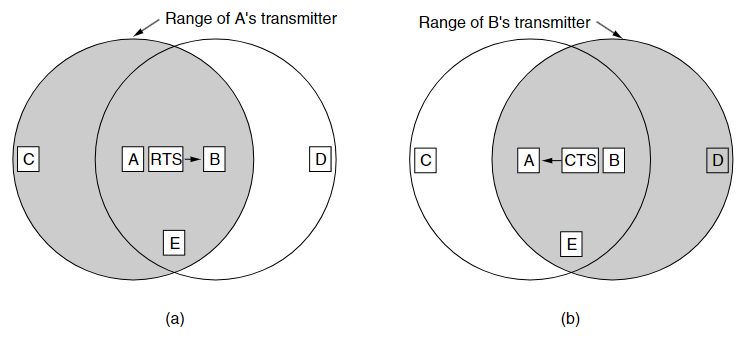
\includegraphics[width=0.309\textwidth]{pic/CN4/The MACA protocol.}
    \caption{The MACA protocol. (a) A sending an RTS to B. (b) B responding with a CTS to A.}
\end{figure}
\begin{itemize}
    \item 任意收到 RTS 的站点需要等待一个时间来保证 A 接受了 CTS. 
    \item 任意收到 CTS 的站点需要保持静默直到数据传输完成, 静默时间可以由CTS中信息决定. 
\end{itemize}

\subsection{Ethernet(IEEE 802.3)}
Two kinds of Ethernet exist
\begin{itemize}
    \item Classical Ethernet: 3 to 10 Mbps
    \item Switched Ethernet: runs at 100, 1000 and 10,000 Mbps
\end{itemize}
Over the cables, information was sent using \textbf{the Manchester encoding}.
\begin{figure}[!htb]
    \centering
    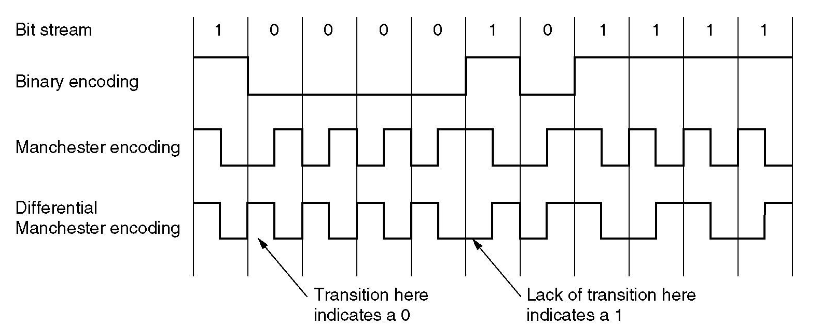
\includegraphics[width=0.42\textwidth]{pic/CN4/the Manchester encoding}
    \caption{the Manchester encoding}
\end{figure}

Ethernet brief history:
\begin{enumerate}
    \item In the mid-1970s, a bus topology. (A broadcast LAN)
    \item By the late 1990s, a hub-based star topology. A hub is a physical layer device. (A broadcast LAN)
    \item In the early 2000s, a switch --- a switch-based star topology (switched Ethernet). A switch is a link layer device. Modern switches are full-duplex. In a switch-base Ethernet LAN there are no collisions. 
\end{enumerate}


Ethernet is by far the most prevalent wired LAN technology. All of the Ethernet technologies provide \textbf{connectionless service} to the network layer.

\subsubsection{Ethernet Frame Structure}
\begin{figure}[!htb]
    \centering
    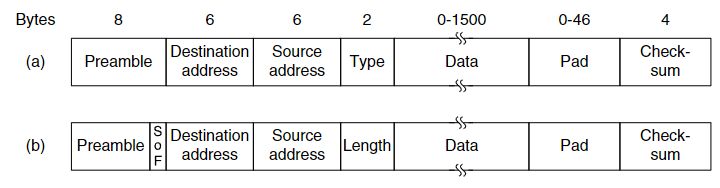
\includegraphics[width=0.42\textwidth]{pic/CN4/Frame formats}
    \caption{Ethernet Frame formats. (a) Ethernet (DIX). (b) IEEE 802.3.}
\end{figure}
\begin{itemize}
    \item \textbf{Preamble}: 8 bytes, each containing the bit pattern
    10101010 (In 802.3, is 10101011). The last byte is called \textbf{the Start of Frame} delimiter for 802.3. It produces a 10-MHz square
    wave, allow the receiver's clock to \textbf{synchronize}. 
    \item \textbf{Two addresses} (MAC addresses): 6*2 bytes. 
    \subitem The first transmitted bit of the destination address is a 0 for ordinary addresses and a 1 for group addresses. 
    \subitem The special address consisting of all 1 bits is reserved for broadcasting. 
    \subitem The 48-bit number of source address. The first 3 bytes of the address field are assigned by IEEE(IEEE 给网卡制造商分配的). The last 3 bytes of the address and programs the complete address into the NIC(网卡制造商烧录进网卡的 id).
    \item The \textbf{Type or Length} field: 2 bytes
    \subitem Any number there less than or equal to 0x600 (1536) can be interpreted as Length, and any number greater than 0x600 can be
    interpreted as Type. 
    \subitem a type code of 0x0800 means that the data contains an IPv4 packet.
    \item The Data field: 46 to 1500 bytes. 
    \subitem This field carries the IP datagram. The maximum transmission unit (MTU) of Ethernet is 1500 bytes. 
    \subitem The minimum size of the data is 46 bytes. Ethernet 要求 from destination address to checksum 的 valid frame 长度必须至少为64 bytes. 
    \begin{figure}[!htb]
        \centering
        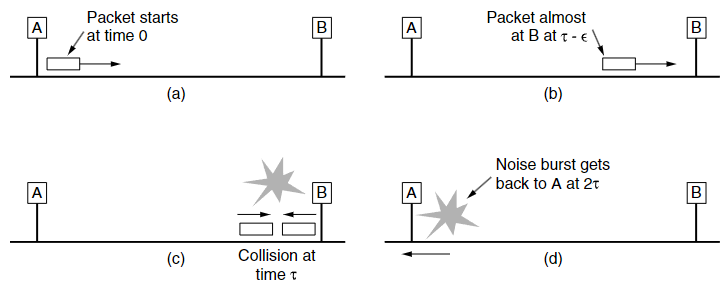
\includegraphics[width=0.42\textwidth]{pic/CN4/Collision detection}
        \caption{Collision detection can take as long as $2\tau$}
    \end{figure}
    \item \textbf{Checksum}: a 32-bit CRC
\end{itemize}

\subsubsection{CSMA/CD with Binary Exponential Backoff}
Classic Ethernet uses the 1-persistent CSMA/CD algorithm. 

How the random interval is determined when a collision occurs?%TODO 重点, 例子 P67
\begin{enumerate}
    \item After a collision
    \item After $i$ collision
    \item After $10$ collision
    \item After $16$ collision, the controller \textit{throws in the towel}(不干了) and reports failure back to the computer. 
\end{enumerate}

\subsubsection{Ethernet Performance}
Ethernet under conditions of heavy and constant load with $k$ stations always ready to transmit.

If each station transmits during a contention slot with probability $p$, the probability $A$ that some station acquires the channel in that slot is 
\begin{align*}
    A=kp(1-p)^{k-1}
\end{align*}
$A$ is maximized when $p=\frac{1}{k}$, with $A\to \frac{1}{e}$ as $k\to\infty$. 

The probability that the contention interval has exactly $j$ slots in it is $A(1-A)^{j-1}$, so the mean number of slots per contention is given by
\begin{align*}
    \sum_{j=0}^\infty jA(1-A)^{j-1}=\frac{1}{A}
\end{align*}
%TODO P69 是上述两式的具体推导. 

Since each slot has a duration $2\tau$, the mean contention interval $w=\frac{2\tau}{A}$. 

If the mean frame takes $P$ sec to transmit,  transmit, when many stations have frames to send
\begin{align*}
    \text{Channel efficiency}=\frac{P}{P+\frac{2\tau}{A}}
\end{align*}
The longer the cable, the longer the contention interval. 

In terms of the frame length, F, the network bandwidth, B, the cable length, L, and the speed of signal propagation, c, for the optimal case of e contention slots per frame. With $P=\frac{F}{B}$, 
\begin{align*}
    \text{Channel efficiency}=\frac{1}{1+\frac{2BLe}{cF}}
\end{align*}
\begin{figure}[!htb]
    \centering
    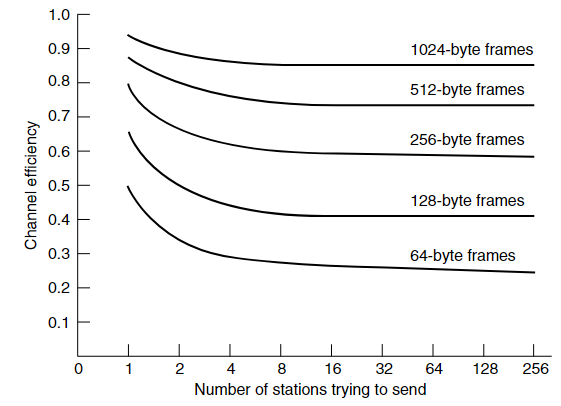
\includegraphics[width=0.309\textwidth]{pic/CN4/Efficiency of Ethernet}
    \caption{Efficiency of Ethernet at 10 Mbps with 512-bit slot times.}
\end{figure}%TODO 修 P -71

\subsubsection{Switched Ethernet}
\begin{figure}[!htb]
    \centering
    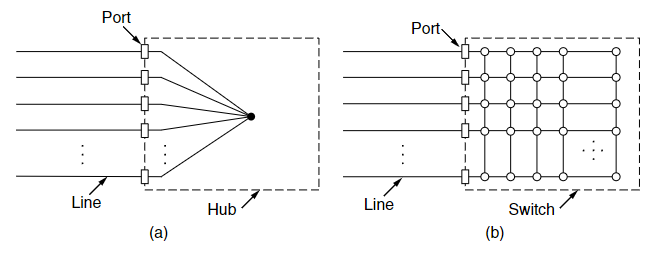
\includegraphics[width=0.42\textwidth]{pic/CN4/Hub and Switch}
    \caption{ (a) Hub. (b) Switch.}
\end{figure}

In a hub, all stations are in the same collision domain. But in a switch, each port is its own independent collision domain.
\begin{figure}[!htb]
    \centering
    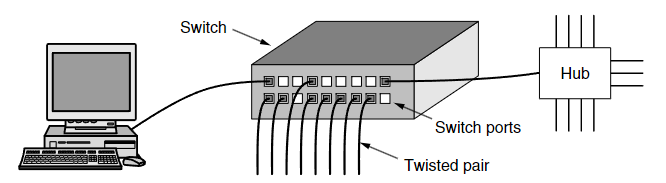
\includegraphics[width=0.42\textwidth]{pic/CN4/An Ethernet switch}
    \caption{An Ethernet switch}
\end{figure}

\subsubsection{Ethernet Technologies}
There are many other Ethernet technologies have been standardized over the years by the IEEE 802.3 CSMA/CD (Ethernet) working group.

e.g. 10BASE-T, 10BASE-2, 100BASE-T, 1000BASE-LX and 10GBASE-T. 

Ethernet is both a link-layer and a physical-layer specification. 

\subsubsection{Gigabit Ethernet}
All configurations of gigabit Ethernet use point-to-point links. 

supports two different modes of operation: 
\begin{itemize}
    \item full-duplex mode: there is a central switch connected to computers. 
    \item half-duplex mode: the computers are connected to a hub
    \subitem Carrier extension: at least 512 bytes
    \subitem Frame bursting
\end{itemize}

\subsection{Wireless LANS (802.11 WiFi)}
802.11 networks can be used in two modes
\begin{itemize}
    \item In infrastructure mode, each client is associated with an AP (Access Point), and APs may be connected together by a wired network
    \item Ad hoc network, there is no access point, and each computer can sent frames to each other directly.
\end{itemize}
\begin{figure}[!htb]
    \centering
    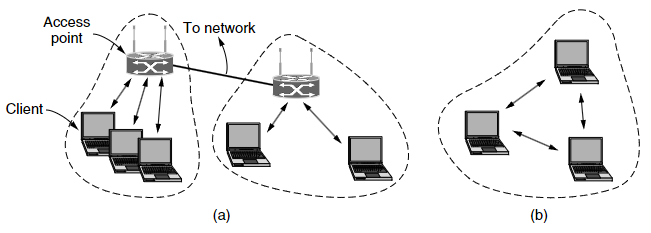
\includegraphics[width=0.42\textwidth]{pic/CN4/802.11 architecture}
    \caption{802.11 architecture. (a) Infrastructure mode. (b) Ad-hoc mode.}
\end{figure}

The data link layer in all the 802.11 protocols is split into two or more sublayers:
\begin{itemize}
    \item The MAC (Medium Access Control)
    \item The LLC (Logical Link Layer)
\end{itemize}
\begin{figure}[!htb]
    \centering
    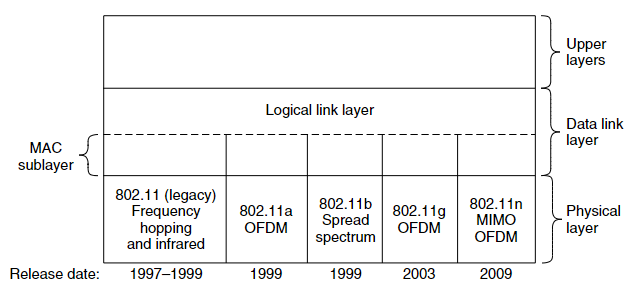
\includegraphics[width=0.42\textwidth]{pic/CN4/Part of the 802.11 protocol stack}
    \caption{Part of the 802.11 protocol stack}
\end{figure}

\subsubsection{802.11 Physical Layer}
Either the 2.4 GHz or the 5GHz ISM (Industrial, Scientific and Medical) frequency bands. 

%TODO 回顾专有名词/缩写

\subsubsection{The 802.11 MAC Sublayer Protocol}
Problems with wireless:
\begin{itemize}
    \item Half duplex: cannot transmit and listen for noise bursts at the same time on a single frequency
    \item Limited Range: The hidden station problem and the exposed station problem    
\end{itemize}
\begin{figure}[!htb]
    \centering
    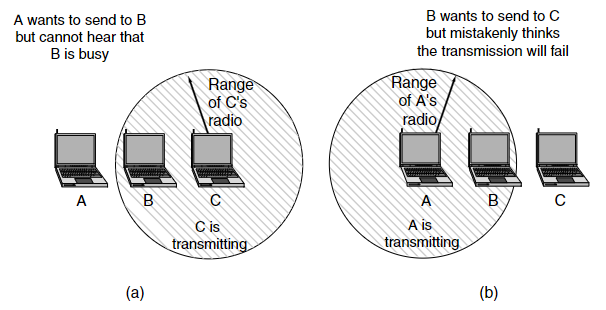
\includegraphics[width=0.42\textwidth]{pic/CN4/Problems with wireless}
    \caption{(a) The hidden terminal problem. (b) The exposed terminal problem.}
\end{figure}

The 802.11 tries to avoid collision with a protocol called CSMA/CA (CSMA with Collision Avoidance).
\begin{itemize}
    \item Channel sensing before sending
    \item Exponential backoff after collision
\end{itemize}
\begin{figure}[!htb]
    \centering
    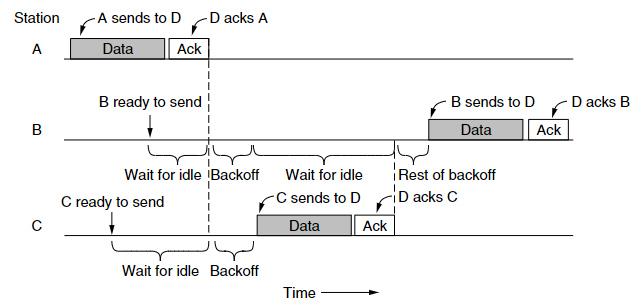
\includegraphics[width=0.42\textwidth]{pic/CN4/Sending a frame with CSMACA}
    \caption{Sending a frame with CSMA/CA. (A, B and C want to send frames to D.)}
\end{figure}


Compared to Ethernet, there are main two differences:
\begin{enumerate}
    \item starting backoffs early helps to avoid collision
    \item acknowledgements are used to infer collision( collision cannot be detected.)
\end{enumerate}

Two modes of operations (backoff):
\begin{enumerate}
    \item DCF (Distributed Coordination Function) because each station acts independently.
    \item PCF (Point Coordinate Function) in which the AP may act as the BS in the cellular network.
\end{enumerate}

To reduce ambiguities about which station is sending, 802.11 defines channel sensing to consists of physical sensing and virtual sensing.
\begin{enumerate}
    \item [Method 1] Physical sensing
    \begin{itemize}
        \item  If idle, just starts transmitting. Does not sense channel while transmitting.
        \item If collision occurs, wait random time, using Ethernet binary exponential backoff algorithm    
    \end{itemize}
    Be used to transmit RTS frame.
    \item [Method 2] Virtual Sensing
    \subitem Scenario: A wants to send to B. C is a station within range of A. D is a station within range of B but not within range of A. (C A B D)
    \begin{figure}[!htb]
        \centering
        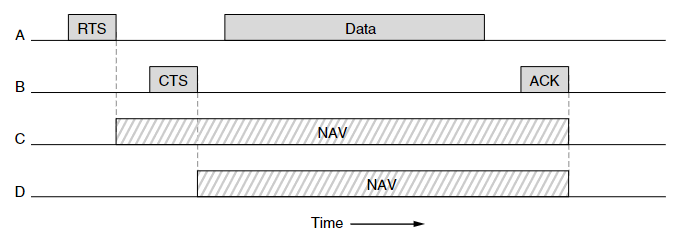
\includegraphics[width=0.42\textwidth]{pic/CN4/Virtual channel sensing using CSMACA}
        \caption{Virtual channel sensing using CSMA/CA}
    \end{figure}

    Note: the NAV signals are NOT transmitted; they are just internal reminder to keep quiet for a certain period of time.
\end{enumerate}

There are several other mechanisms to improve its performance:
\begin{enumerate}
    \item Reliability
    \subitem To lower the transmission rate. send shorter frames, allow frames to be split into smaller pieces, called fragments. 
    \item Power: the basic mechanism for saving power builds on beacon frames
    \item Quality of Services: After a frame has been sent, a certain amount of idle time is required before any station may send a frame to check that the channel is no longer in use. 
\end{enumerate}

\subsubsection{The 802.11 Frame Structure}
The 802.11 standard defines three different classes of frames in the air: data, control, and management. 
\begin{figure}[!htb]
    \centering
    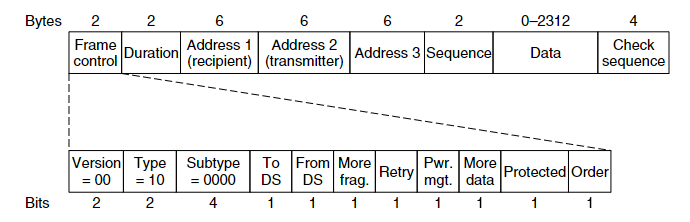
\includegraphics[width=0.42\textwidth]{pic/CN4/Format of the 802.11 data frame}
    \caption{Format of the 802.11 data frame}
\end{figure}

\begin{itemize}
    \item data frame
    \begin{itemize}
        \item Address fields: data frames sent to or from an AP, but the AP may be a relay point, so the Address 3 gives a distant destination.
        \item Protocol Version: set to 00
        \item Type: data, control, or management; Subtype: RTS, CTS, or ACK of control frame; for a regular data frame (without quality of service), they are set to 10 and 0000 in binary.
        \item To DS and From DS: to indicate whether the fame is going to or coming from the networks connected to the APs.
        \item More Fragments: more fragments will follow;
        \item Retry: retransmission;
        \item Pwr: sleep state;
        \item More data: sender has additional frames;
        \item The Protected Frame bit: encrypted usign WEP;
        \item The Order bit: processed strictly in order;
        \item Duration: time the frame and its acknowledgement takes; it also exists in control frame.
        \item Sequence: 16 bits, 12 for frame, 4 for fragment.
    \end{itemize}
    \item Management frames: similar to data frames, except without one of the base station addresses, because management frames are restricted to a single cell.
    \item Control frames: shorter
\end{itemize}

Each 802.11 LAN must provide nine services

\subsection{Data Link Layer Switching}
We can treat one physical LAN as multiple logical LANs, called
VLANs (Virtual LANs)

\subsubsection{Learning Bridge}%TODO 之后摸了 P101
All of the stations attached to the same port on a bridge belong to the same collision domain. 

%TODO 补图

have a big (hash) table. This table can list each possible destination and which output port it belongs to.  use a flooding algorithm:
\begin{itemize}
    \item Every incoming frame for an unknown destination is output on all the ports to
    which the bridge is connected except the one it arrived on
    \item Once a destination is known, frames destined for it are put only on the proper port
\end{itemize}

By looking at the source addresses, they can tell which machines are accessible on which ports. 

But the network topology is dynamic. To handle it, the arrival time of the frame is noted in the entry. 

Periodically, a process in the bridge scans the hash table and purges all entries more than a few minutes old.

The routing:
\begin{enumerate}
    \item If the port for the destination address is the same as the source port, discard the frame.
    \item If the port for the destination address and the source port are different, forward the frame on to the destination port.
    \item If the destination port is unknown, use flooding and send the frame on all ports except the source port.
\end{enumerate}

\subsubsection{Protocol Processing at a Bridge}
In the general case, relays at a given layer can rewrite the headers for that layer.

%TODO 补图, P 106

e.g. %图 P107

\subsubsection{Spanning Tree Bridges}% P108-


\paragraph{Spanning Tree Algorithm}

% e.g. 跳过吧


\subsection{Repeaters, Hubs, Bridges, Switches, Routers, and Gateways}%TODO P119
The layer matters because different devices use different pieces of information to decide how to switch

\subsubsection{Repeaters and Hubs (Physical Layer)}

\subsubsection{Bridges and Switches (Data Link Layer)}

\subsubsection{Routers (Network Layer)}

\subsubsection{Gateways}

\subsubsection{Virtual LANs}